\documentclass{article} % For LaTeX2e
\usepackage{iclr2019_conference,times}

% Optional math commands from https://github.com/goodfeli/dlbook_notation.
%%%%% NEW MATH DEFINITIONS %%%%%

\usepackage{amsmath,amsfonts,bm}

% Mark sections of captions for referring to divisions of figures
\newcommand{\figleft}{{\em (Left)}}
\newcommand{\figcenter}{{\em (Center)}}
\newcommand{\figright}{{\em (Right)}}
\newcommand{\figtop}{{\em (Top)}}
\newcommand{\figbottom}{{\em (Bottom)}}
\newcommand{\captiona}{{\em (a)}}
\newcommand{\captionb}{{\em (b)}}
\newcommand{\captionc}{{\em (c)}}
\newcommand{\captiond}{{\em (d)}}

% Highlight a newly defined term
\newcommand{\newterm}[1]{{\bf #1}}


% Figure reference, lower-case.
\def\figref#1{figure~\ref{#1}}
% Figure reference, capital. For start of sentence
\def\Figref#1{Figure~\ref{#1}}
\def\twofigref#1#2{figures \ref{#1} and \ref{#2}}
\def\quadfigref#1#2#3#4{figures \ref{#1}, \ref{#2}, \ref{#3} and \ref{#4}}
% Section reference, lower-case.
\def\secref#1{section~\ref{#1}}
% Section reference, capital.
\def\Secref#1{Section~\ref{#1}}
% Reference to two sections.
\def\twosecrefs#1#2{sections \ref{#1} and \ref{#2}}
% Reference to three sections.
\def\secrefs#1#2#3{sections \ref{#1}, \ref{#2} and \ref{#3}}
% Reference to an equation, lower-case.
\def\eqref#1{equation~\ref{#1}}
% Reference to an equation, upper case
\def\Eqref#1{Equation~\ref{#1}}
% A raw reference to an equation---avoid using if possible
\def\plaineqref#1{\ref{#1}}
% Reference to a chapter, lower-case.
\def\chapref#1{chapter~\ref{#1}}
% Reference to an equation, upper case.
\def\Chapref#1{Chapter~\ref{#1}}
% Reference to a range of chapters
\def\rangechapref#1#2{chapters\ref{#1}--\ref{#2}}
% Reference to an algorithm, lower-case.
\def\algref#1{algorithm~\ref{#1}}
% Reference to an algorithm, upper case.
\def\Algref#1{Algorithm~\ref{#1}}
\def\twoalgref#1#2{algorithms \ref{#1} and \ref{#2}}
\def\Twoalgref#1#2{Algorithms \ref{#1} and \ref{#2}}
% Reference to a part, lower case
\def\partref#1{part~\ref{#1}}
% Reference to a part, upper case
\def\Partref#1{Part~\ref{#1}}
\def\twopartref#1#2{parts \ref{#1} and \ref{#2}}

\def\ceil#1{\lceil #1 \rceil}
\def\floor#1{\lfloor #1 \rfloor}
\def\1{\bm{1}}
\newcommand{\train}{\mathcal{D}}
\newcommand{\valid}{\mathcal{D_{\mathrm{valid}}}}
\newcommand{\test}{\mathcal{D_{\mathrm{test}}}}

\def\eps{{\epsilon}}


% Random variables
\def\reta{{\textnormal{$\eta$}}}
\def\ra{{\textnormal{a}}}
\def\rb{{\textnormal{b}}}
\def\rc{{\textnormal{c}}}
\def\rd{{\textnormal{d}}}
\def\re{{\textnormal{e}}}
\def\rf{{\textnormal{f}}}
\def\rg{{\textnormal{g}}}
\def\rh{{\textnormal{h}}}
\def\ri{{\textnormal{i}}}
\def\rj{{\textnormal{j}}}
\def\rk{{\textnormal{k}}}
\def\rl{{\textnormal{l}}}
% rm is already a command, just don't name any random variables m
\def\rn{{\textnormal{n}}}
\def\ro{{\textnormal{o}}}
\def\rp{{\textnormal{p}}}
\def\rq{{\textnormal{q}}}
\def\rr{{\textnormal{r}}}
\def\rs{{\textnormal{s}}}
\def\rt{{\textnormal{t}}}
\def\ru{{\textnormal{u}}}
\def\rv{{\textnormal{v}}}
\def\rw{{\textnormal{w}}}
\def\rx{{\textnormal{x}}}
\def\ry{{\textnormal{y}}}
\def\rz{{\textnormal{z}}}

% Random vectors
\def\rvepsilon{{\mathbf{\epsilon}}}
\def\rvtheta{{\mathbf{\theta}}}
\def\rva{{\mathbf{a}}}
\def\rvb{{\mathbf{b}}}
\def\rvc{{\mathbf{c}}}
\def\rvd{{\mathbf{d}}}
\def\rve{{\mathbf{e}}}
\def\rvf{{\mathbf{f}}}
\def\rvg{{\mathbf{g}}}
\def\rvh{{\mathbf{h}}}
\def\rvu{{\mathbf{i}}}
\def\rvj{{\mathbf{j}}}
\def\rvk{{\mathbf{k}}}
\def\rvl{{\mathbf{l}}}
\def\rvm{{\mathbf{m}}}
\def\rvn{{\mathbf{n}}}
\def\rvo{{\mathbf{o}}}
\def\rvp{{\mathbf{p}}}
\def\rvq{{\mathbf{q}}}
\def\rvr{{\mathbf{r}}}
\def\rvs{{\mathbf{s}}}
\def\rvt{{\mathbf{t}}}
\def\rvu{{\mathbf{u}}}
\def\rvv{{\mathbf{v}}}
\def\rvw{{\mathbf{w}}}
\def\rvx{{\mathbf{x}}}
\def\rvy{{\mathbf{y}}}
\def\rvz{{\mathbf{z}}}

% Elements of random vectors
\def\erva{{\textnormal{a}}}
\def\ervb{{\textnormal{b}}}
\def\ervc{{\textnormal{c}}}
\def\ervd{{\textnormal{d}}}
\def\erve{{\textnormal{e}}}
\def\ervf{{\textnormal{f}}}
\def\ervg{{\textnormal{g}}}
\def\ervh{{\textnormal{h}}}
\def\ervi{{\textnormal{i}}}
\def\ervj{{\textnormal{j}}}
\def\ervk{{\textnormal{k}}}
\def\ervl{{\textnormal{l}}}
\def\ervm{{\textnormal{m}}}
\def\ervn{{\textnormal{n}}}
\def\ervo{{\textnormal{o}}}
\def\ervp{{\textnormal{p}}}
\def\ervq{{\textnormal{q}}}
\def\ervr{{\textnormal{r}}}
\def\ervs{{\textnormal{s}}}
\def\ervt{{\textnormal{t}}}
\def\ervu{{\textnormal{u}}}
\def\ervv{{\textnormal{v}}}
\def\ervw{{\textnormal{w}}}
\def\ervx{{\textnormal{x}}}
\def\ervy{{\textnormal{y}}}
\def\ervz{{\textnormal{z}}}

% Random matrices
\def\rmA{{\mathbf{A}}}
\def\rmB{{\mathbf{B}}}
\def\rmC{{\mathbf{C}}}
\def\rmD{{\mathbf{D}}}
\def\rmE{{\mathbf{E}}}
\def\rmF{{\mathbf{F}}}
\def\rmG{{\mathbf{G}}}
\def\rmH{{\mathbf{H}}}
\def\rmI{{\mathbf{I}}}
\def\rmJ{{\mathbf{J}}}
\def\rmK{{\mathbf{K}}}
\def\rmL{{\mathbf{L}}}
\def\rmM{{\mathbf{M}}}
\def\rmN{{\mathbf{N}}}
\def\rmO{{\mathbf{O}}}
\def\rmP{{\mathbf{P}}}
\def\rmQ{{\mathbf{Q}}}
\def\rmR{{\mathbf{R}}}
\def\rmS{{\mathbf{S}}}
\def\rmT{{\mathbf{T}}}
\def\rmU{{\mathbf{U}}}
\def\rmV{{\mathbf{V}}}
\def\rmW{{\mathbf{W}}}
\def\rmX{{\mathbf{X}}}
\def\rmY{{\mathbf{Y}}}
\def\rmZ{{\mathbf{Z}}}

% Elements of random matrices
\def\ermA{{\textnormal{A}}}
\def\ermB{{\textnormal{B}}}
\def\ermC{{\textnormal{C}}}
\def\ermD{{\textnormal{D}}}
\def\ermE{{\textnormal{E}}}
\def\ermF{{\textnormal{F}}}
\def\ermG{{\textnormal{G}}}
\def\ermH{{\textnormal{H}}}
\def\ermI{{\textnormal{I}}}
\def\ermJ{{\textnormal{J}}}
\def\ermK{{\textnormal{K}}}
\def\ermL{{\textnormal{L}}}
\def\ermM{{\textnormal{M}}}
\def\ermN{{\textnormal{N}}}
\def\ermO{{\textnormal{O}}}
\def\ermP{{\textnormal{P}}}
\def\ermQ{{\textnormal{Q}}}
\def\ermR{{\textnormal{R}}}
\def\ermS{{\textnormal{S}}}
\def\ermT{{\textnormal{T}}}
\def\ermU{{\textnormal{U}}}
\def\ermV{{\textnormal{V}}}
\def\ermW{{\textnormal{W}}}
\def\ermX{{\textnormal{X}}}
\def\ermY{{\textnormal{Y}}}
\def\ermZ{{\textnormal{Z}}}

% Vectors
\def\vzero{{\bm{0}}}
\def\vone{{\bm{1}}}
\def\vmu{{\bm{\mu}}}
\def\vtheta{{\bm{\theta}}}
\def\va{{\bm{a}}}
\def\vb{{\bm{b}}}
\def\vc{{\bm{c}}}
\def\vd{{\bm{d}}}
\def\ve{{\bm{e}}}
\def\vf{{\bm{f}}}
\def\vg{{\bm{g}}}
\def\vh{{\bm{h}}}
\def\vi{{\bm{i}}}
\def\vj{{\bm{j}}}
\def\vk{{\bm{k}}}
\def\vl{{\bm{l}}}
\def\vm{{\bm{m}}}
\def\vn{{\bm{n}}}
\def\vo{{\bm{o}}}
\def\vp{{\bm{p}}}
\def\vq{{\bm{q}}}
\def\vr{{\bm{r}}}
\def\vs{{\bm{s}}}
\def\vt{{\bm{t}}}
\def\vu{{\bm{u}}}
\def\vv{{\bm{v}}}
\def\vw{{\bm{w}}}
\def\vx{{\bm{x}}}
\def\vy{{\bm{y}}}
\def\vz{{\bm{z}}}

% Elements of vectors
\def\evalpha{{\alpha}}
\def\evbeta{{\beta}}
\def\evepsilon{{\epsilon}}
\def\evlambda{{\lambda}}
\def\evomega{{\omega}}
\def\evmu{{\mu}}
\def\evpsi{{\psi}}
\def\evsigma{{\sigma}}
\def\evtheta{{\theta}}
\def\eva{{a}}
\def\evb{{b}}
\def\evc{{c}}
\def\evd{{d}}
\def\eve{{e}}
\def\evf{{f}}
\def\evg{{g}}
\def\evh{{h}}
\def\evi{{i}}
\def\evj{{j}}
\def\evk{{k}}
\def\evl{{l}}
\def\evm{{m}}
\def\evn{{n}}
\def\evo{{o}}
\def\evp{{p}}
\def\evq{{q}}
\def\evr{{r}}
\def\evs{{s}}
\def\evt{{t}}
\def\evu{{u}}
\def\evv{{v}}
\def\evw{{w}}
\def\evx{{x}}
\def\evy{{y}}
\def\evz{{z}}

% Matrix
\def\mA{{\bm{A}}}
\def\mB{{\bm{B}}}
\def\mC{{\bm{C}}}
\def\mD{{\bm{D}}}
\def\mE{{\bm{E}}}
\def\mF{{\bm{F}}}
\def\mG{{\bm{G}}}
\def\mH{{\bm{H}}}
\def\mI{{\bm{I}}}
\def\mJ{{\bm{J}}}
\def\mK{{\bm{K}}}
\def\mL{{\bm{L}}}
\def\mM{{\bm{M}}}
\def\mN{{\bm{N}}}
\def\mO{{\bm{O}}}
\def\mP{{\bm{P}}}
\def\mQ{{\bm{Q}}}
\def\mR{{\bm{R}}}
\def\mS{{\bm{S}}}
\def\mT{{\bm{T}}}
\def\mU{{\bm{U}}}
\def\mV{{\bm{V}}}
\def\mW{{\bm{W}}}
\def\mX{{\bm{X}}}
\def\mY{{\bm{Y}}}
\def\mZ{{\bm{Z}}}
\def\mBeta{{\bm{\beta}}}
\def\mPhi{{\bm{\Phi}}}
\def\mLambda{{\bm{\Lambda}}}
\def\mSigma{{\bm{\Sigma}}}

% Tensor
\DeclareMathAlphabet{\mathsfit}{\encodingdefault}{\sfdefault}{m}{sl}
\SetMathAlphabet{\mathsfit}{bold}{\encodingdefault}{\sfdefault}{bx}{n}
\newcommand{\tens}[1]{\bm{\mathsfit{#1}}}
\def\tA{{\tens{A}}}
\def\tB{{\tens{B}}}
\def\tC{{\tens{C}}}
\def\tD{{\tens{D}}}
\def\tE{{\tens{E}}}
\def\tF{{\tens{F}}}
\def\tG{{\tens{G}}}
\def\tH{{\tens{H}}}
\def\tI{{\tens{I}}}
\def\tJ{{\tens{J}}}
\def\tK{{\tens{K}}}
\def\tL{{\tens{L}}}
\def\tM{{\tens{M}}}
\def\tN{{\tens{N}}}
\def\tO{{\tens{O}}}
\def\tP{{\tens{P}}}
\def\tQ{{\tens{Q}}}
\def\tR{{\tens{R}}}
\def\tS{{\tens{S}}}
\def\tT{{\tens{T}}}
\def\tU{{\tens{U}}}
\def\tV{{\tens{V}}}
\def\tW{{\tens{W}}}
\def\tX{{\tens{X}}}
\def\tY{{\tens{Y}}}
\def\tZ{{\tens{Z}}}


% Graph
\def\gA{{\mathcal{A}}}
\def\gB{{\mathcal{B}}}
\def\gC{{\mathcal{C}}}
\def\gD{{\mathcal{D}}}
\def\gE{{\mathcal{E}}}
\def\gF{{\mathcal{F}}}
\def\gG{{\mathcal{G}}}
\def\gH{{\mathcal{H}}}
\def\gI{{\mathcal{I}}}
\def\gJ{{\mathcal{J}}}
\def\gK{{\mathcal{K}}}
\def\gL{{\mathcal{L}}}
\def\gM{{\mathcal{M}}}
\def\gN{{\mathcal{N}}}
\def\gO{{\mathcal{O}}}
\def\gP{{\mathcal{P}}}
\def\gQ{{\mathcal{Q}}}
\def\gR{{\mathcal{R}}}
\def\gS{{\mathcal{S}}}
\def\gT{{\mathcal{T}}}
\def\gU{{\mathcal{U}}}
\def\gV{{\mathcal{V}}}
\def\gW{{\mathcal{W}}}
\def\gX{{\mathcal{X}}}
\def\gY{{\mathcal{Y}}}
\def\gZ{{\mathcal{Z}}}

% Sets
\def\sA{{\mathbb{A}}}
\def\sB{{\mathbb{B}}}
\def\sC{{\mathbb{C}}}
\def\sD{{\mathbb{D}}}
% Don't use a set called E, because this would be the same as our symbol
% for expectation.
\def\sF{{\mathbb{F}}}
\def\sG{{\mathbb{G}}}
\def\sH{{\mathbb{H}}}
\def\sI{{\mathbb{I}}}
\def\sJ{{\mathbb{J}}}
\def\sK{{\mathbb{K}}}
\def\sL{{\mathbb{L}}}
\def\sM{{\mathbb{M}}}
\def\sN{{\mathbb{N}}}
\def\sO{{\mathbb{O}}}
\def\sP{{\mathbb{P}}}
\def\sQ{{\mathbb{Q}}}
\def\sR{{\mathbb{R}}}
\def\sS{{\mathbb{S}}}
\def\sT{{\mathbb{T}}}
\def\sU{{\mathbb{U}}}
\def\sV{{\mathbb{V}}}
\def\sW{{\mathbb{W}}}
\def\sX{{\mathbb{X}}}
\def\sY{{\mathbb{Y}}}
\def\sZ{{\mathbb{Z}}}

% Entries of a matrix
\def\emLambda{{\Lambda}}
\def\emA{{A}}
\def\emB{{B}}
\def\emC{{C}}
\def\emD{{D}}
\def\emE{{E}}
\def\emF{{F}}
\def\emG{{G}}
\def\emH{{H}}
\def\emI{{I}}
\def\emJ{{J}}
\def\emK{{K}}
\def\emL{{L}}
\def\emM{{M}}
\def\emN{{N}}
\def\emO{{O}}
\def\emP{{P}}
\def\emQ{{Q}}
\def\emR{{R}}
\def\emS{{S}}
\def\emT{{T}}
\def\emU{{U}}
\def\emV{{V}}
\def\emW{{W}}
\def\emX{{X}}
\def\emY{{Y}}
\def\emZ{{Z}}
\def\emSigma{{\Sigma}}

% entries of a tensor
% Same font as tensor, without \bm wrapper
\newcommand{\etens}[1]{\mathsfit{#1}}
\def\etLambda{{\etens{\Lambda}}}
\def\etA{{\etens{A}}}
\def\etB{{\etens{B}}}
\def\etC{{\etens{C}}}
\def\etD{{\etens{D}}}
\def\etE{{\etens{E}}}
\def\etF{{\etens{F}}}
\def\etG{{\etens{G}}}
\def\etH{{\etens{H}}}
\def\etI{{\etens{I}}}
\def\etJ{{\etens{J}}}
\def\etK{{\etens{K}}}
\def\etL{{\etens{L}}}
\def\etM{{\etens{M}}}
\def\etN{{\etens{N}}}
\def\etO{{\etens{O}}}
\def\etP{{\etens{P}}}
\def\etQ{{\etens{Q}}}
\def\etR{{\etens{R}}}
\def\etS{{\etens{S}}}
\def\etT{{\etens{T}}}
\def\etU{{\etens{U}}}
\def\etV{{\etens{V}}}
\def\etW{{\etens{W}}}
\def\etX{{\etens{X}}}
\def\etY{{\etens{Y}}}
\def\etZ{{\etens{Z}}}

% The true underlying data generating distribution
\newcommand{\pdata}{p_{\rm{data}}}
% The empirical distribution defined by the training set
\newcommand{\ptrain}{\hat{p}_{\rm{data}}}
\newcommand{\Ptrain}{\hat{P}_{\rm{data}}}
% The model distribution
\newcommand{\pmodel}{p_{\rm{model}}}
\newcommand{\Pmodel}{P_{\rm{model}}}
\newcommand{\ptildemodel}{\tilde{p}_{\rm{model}}}
% Stochastic autoencoder distributions
\newcommand{\pencode}{p_{\rm{encoder}}}
\newcommand{\pdecode}{p_{\rm{decoder}}}
\newcommand{\precons}{p_{\rm{reconstruct}}}

\newcommand{\laplace}{\mathrm{Laplace}} % Laplace distribution

\newcommand{\E}{\mathbb{E}}
\newcommand{\Ls}{\mathcal{L}}
\newcommand{\R}{\mathbb{R}}
\newcommand{\emp}{\tilde{p}}
\newcommand{\lr}{\alpha}
\newcommand{\reg}{\lambda}
\newcommand{\rect}{\mathrm{rectifier}}
\newcommand{\softmax}{\mathrm{softmax}}
\newcommand{\sigmoid}{\sigma}
\newcommand{\softplus}{\zeta}
\newcommand{\KL}{D_{\mathrm{KL}}}
\newcommand{\Var}{\mathrm{Var}}
\newcommand{\standarderror}{\mathrm{SE}}
\newcommand{\Cov}{\mathrm{Cov}}
% Wolfram Mathworld says $L^2$ is for function spaces and $\ell^2$ is for vectors
% But then they seem to use $L^2$ for vectors throughout the site, and so does
% wikipedia.
\newcommand{\normlzero}{L^0}
\newcommand{\normlone}{L^1}
\newcommand{\normltwo}{L^2}
\newcommand{\normlp}{L^p}
\newcommand{\normmax}{L^\infty}

\newcommand{\parents}{Pa} % See usage in notation.tex. Chosen to match Daphne's book.

\DeclareMathOperator*{\argmax}{arg\,max}
\DeclareMathOperator*{\argmin}{arg\,min}

\DeclareMathOperator{\sign}{sign}
\DeclareMathOperator{\Tr}{Tr}
\let\ab\allowbreak


\usepackage{hyperref}
\usepackage{url}
\usepackage{graphicx}

\title{Reproducibility Challenge: Adjustable Real-Time Style Transfer}

% Authors must not appear in the submitted version. They should be hidden
% as long as the \iclrfinalcopy macro remains commented out below.
% Non-anonymous submissions will be rejected without review.

\author{Rohan Bungre, Carl Richardson, Charlie Steptoe \& Alexander Thomas}

% The \author macro works with any number of authors. There are two commands
% used to separate the names and addresses of multiple authors: \And and \AND.
%
% Using \And between authors leaves it to \LaTeX{} to determine where to break
% the lines. Using \AND forces a linebreak at that point. So, if \LaTeX{}
% puts 3 of 4 authors names on the first line, and the last on the second
% line, try using \AND instead of \And before the third author name.

\newcommand{\fix}{\marginpar{FIX}}
\newcommand{\new}{\marginpar{NEW}}

\iclrfinalcopy % Uncomment for camera-ready version, but NOT for submission.
\begin{document}
\maketitle
\begin{abstract}
\emph{`Adjustable Real-Time Style Transfer' (ICLR 2020) addresses the inclusion of a secondary conditioner network to adjust hyperparameters without retraining a style transfer network, otherwise requiring hours of computation. This document attempts to recreate the paper's findings, by reproducing figures and describing the difficulties and nuances in reproducing the described network. Relevant code can be found at the} Real-Time-Adjustable-Style-Transfer \emph{repository} (git.io/JsT1E)
\end{abstract}

\section{Introduction}
This report evaluates the reproducibility of \cite{babaeizadeh2018adjustable}. Neural Style Transfer traditionally requires retraining of networks whilst varying hyperparameters over many hours to produce sensible results. This recent work optimises a new network that extends the input to include these hyperparameters, thus allowing for real-time tuning to produce variable and more suitable results without retraining. Result reproduction utilised an existing code base for similar problems.

\section{Reproduction of Code}

\subsection{Adapting Existing Code}

To understand the established structure of code for style transfer problems, it was useful to find an existing implementation for previous, similar papers. Investigation yielded an implementation using the PyTorch library, from Nikita Prudnikov. During this work, it was realised that although the basic implementation follows the intentions of the original paper, minute implementation details were overlooked. Incorrect VGG-19 layers were used, with inconsistent use of instance normalisation and exponential moving average compensation on content loss, so manual scale correction was required, the removal of which is the intention of this paper.

\begin{figure}[h!]
\centering
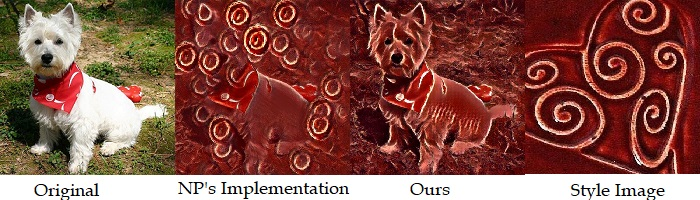
\includegraphics[width=0.7\textwidth]{GitHubvsOwn.jpg}
\vspace{-3mm}
\caption{Initial Results Comparison}
\vspace{1mm}
\label{fig:GitHubvsOwn}
\vspace{-2mm}
\end{figure}

Overall, the original code was found to prioritise style loss and the conditioner network responsible for hyperparameter replacement was less effective than expected, meaning the content image became lost. Regardless, this implementation provided a base to amend and more accurately follow the intended implementation. Example stylised images can be seen in Figure \ref{fig:GitHubvsOwn}, for comparison against the amended version.

\subsection{Implementation Details}

All references to equations and figures made in this section are with respect to \cite{babaeizadeh2018adjustable}. Details of the network architectures were provided in the appendix. The conditioner was comprised of 11 dense layers; however, the output function of each layer was not explicitly stated (like it was for the stylizing network). After our first attempt of replicating the model failed, we assumed ReLU activations were used on all but the output layer, as standard for dense layers. The full architecture of the stylizing network was explicitly stated. The conditional instance normalisation, as given by equation 6, was applied to the output of each activation function following all convolutions.

Equation 1 shows the loss was computed by passing images into a pre-trained network and extracting specific features. There were several discrepancies in this section. From how the loss was detailed, it seemed like equation 1 included a mistake and the content loss at layer \(l\) should be between the activation of the stylized and content images. Furthermore, figure \(2\) indicates VGG-16 was utilised whereas section 5.1 stated VGG-19. The implementation details and VGG-19 was implemented. Finally, the implementation details describes the features extracted as `the last feature set of conv2, conv3 and conv4 layers'. After downloading the pre-trained VGG-19 network from Pytorch, we found these labels didn't map to those used in the module description and we were unable to confidently identify the correct layers and to which `the last feature set' corresponded. We opted to use the $conv2\_2$, $conv3\_3$ \& $conv4\_3$ convolutional layers from the network.

The model was now ready to be trained using the loss and optimisation details specified throughout the paper and in the appendix. However, before this, the training images/data had to be prepared. The paper provided no details of how the images were pre-processed so we decided to re-use the transformations from the existing code. The content images, before input to the stylizing network were resized to 256x256, centre cropped and each pixel value was scaled by 255. This ensured all content images were formatted identically. The style image, before being standardised, had each pixel value scaled by 255. Before passing any image into VGG-19, all pixel values were divided by 255 and each input channel was standardised using the ImageNet means and variances. Regarding the training data, section 5.1 and the appendix provided necessary details, where the appendix details were interpreted as a single epoch using 200,000 batches of size 8.

\subsection{Training, Initial Results \& Loss Values}

\begin{figure}[h!]
    \centering
    \vspace{-1mm}
    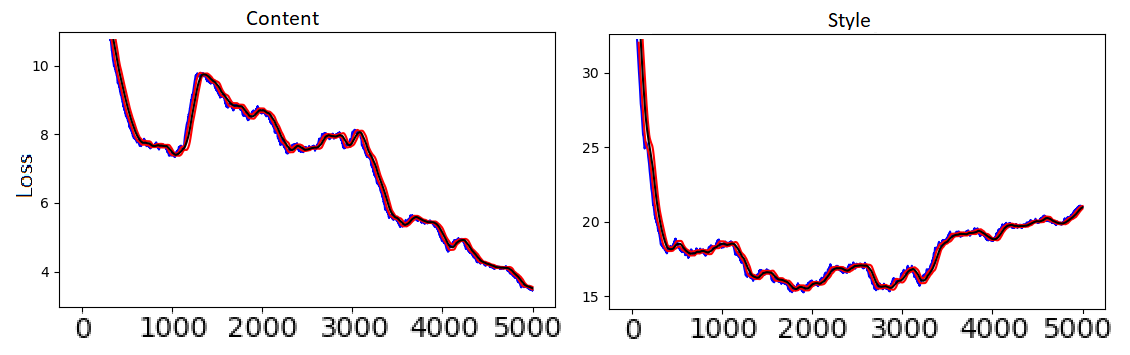
\includegraphics[width=0.6\textwidth]{Saddle.png}
    \vspace{-2mm}
    \caption{Loss Function Saddle Point at Batch $\approx$ 3000}
    \label{fig:loss_saddle}
    \vspace{-3mm}
\end{figure}

In contrast to the existing code, when re-implemented, the networks trained steadily, with a decreasing loss value for both style and content. However, at approximately batch 3000 of training, the loss function appeared to reach a saddle point. Beyond this, the content loss dropped dramatically and the style loss rose, as seen in Figure \ref{fig:loss_saddle}. This may be due to sharing of VGG-19 layers between content and style. As a result, supervision was required to ensure this did not occur.

The trained revised network produced considerably more convincing results, though it is arguable that it learned a content loss that was too low, resulting in less variety. The two implementations' outputs can be seen in Figure \ref{fig:GitHubvsOwn}. Each new style image used requires 200,000 epochs to adhere strictly to the ICLR paper ($\sim$ 25 hours), so it was decided to use only the most common style.

\section{Figure Reproducibility}

\subsection{Layer Loss}

Figure 7 in \cite{babaeizadeh2018adjustable} encapsulates main motivation of the original ICLR paper. It is clear that by adjusting the input $\boldsymbol{\alpha}$ vector, the respective loss of that layer of the VGG-19 network should decrease when compared against a style image. This behaviour facilitates the \emph{real-time adjustable} nature of the network. The network was passed an image and the input $\boldsymbol{\alpha}$ vector elements varied individually between zero and one, whilst keeping the other elements constant at zero or one. The reproduced plot using our implementation can be seen in Figure \ref{fig:layer_loss}. Note that, unexpectedly some layer losses, in fact, increase with their respective $\alpha$ value. It is not clear why this is the case, but it may correlate with findings of Section \ref{ss:noise}.

\begin{figure}[h!]
    \centering
    \vspace{-1mm}
    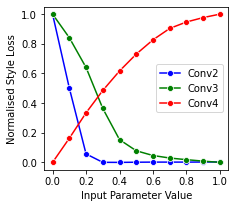
\includegraphics[width=0.25\textwidth]{zeros.png}
    \hspace{0.5cm}
    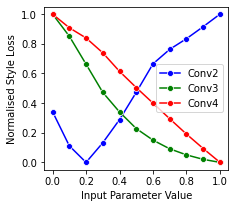
\includegraphics[width=0.25\textwidth]{ones.png}
    \vspace{-4mm}
    \caption{Layer Loss Plots w/ Remaining $\alpha_s$ kept at 0 (Left) and 1 (Right)}
    \label{fig:layer_loss}
    \vspace{-5mm}
\end{figure}

\subsection{Varying the Image Style}\label{ss:style}
When reproducing Figures 3 and 6 from \cite{babaeizadeh2018adjustable}, several issues as no source images were defined, nor their scale. Testing found that the size of the input image affected the styling of the output image. Using reverse image search, the original test images were found and scaled down to a size of (300x300) for optimal results. The first experiment was to reproduce the effect of adjusting input parameters on stylisation (Figure 3). The stylised output was observed with a given layer weight increasing from 0 to 1, with the rest fixed to 0. The details of each stylisation should vary with weights as deeper layers represent larger features of the style image.

Using Prudnikov's model, the input image was stylised, and intensity of stylisation did increase as with increased weights, shown in Figure \ref{fig3}. However, it is unclear from this reproduction if deeper layers used larger features of the style image to stylise the content. A major issue with this model was that when all style weights were 0, content image reconstruction was imperfect. Using the group's model, the input image was stylised and again, stylisation did increase with increased weights as shown in Figure \ref{fig3}. Unlike the previous model, the deeper layer (conv\_3) does use larger features to style the image, when compared to (conv\_2). The problem with the group's model was that the deepest layer (conv\_4) was not contributing any style to the image.

\begin{figure}[h!]
    \centering
    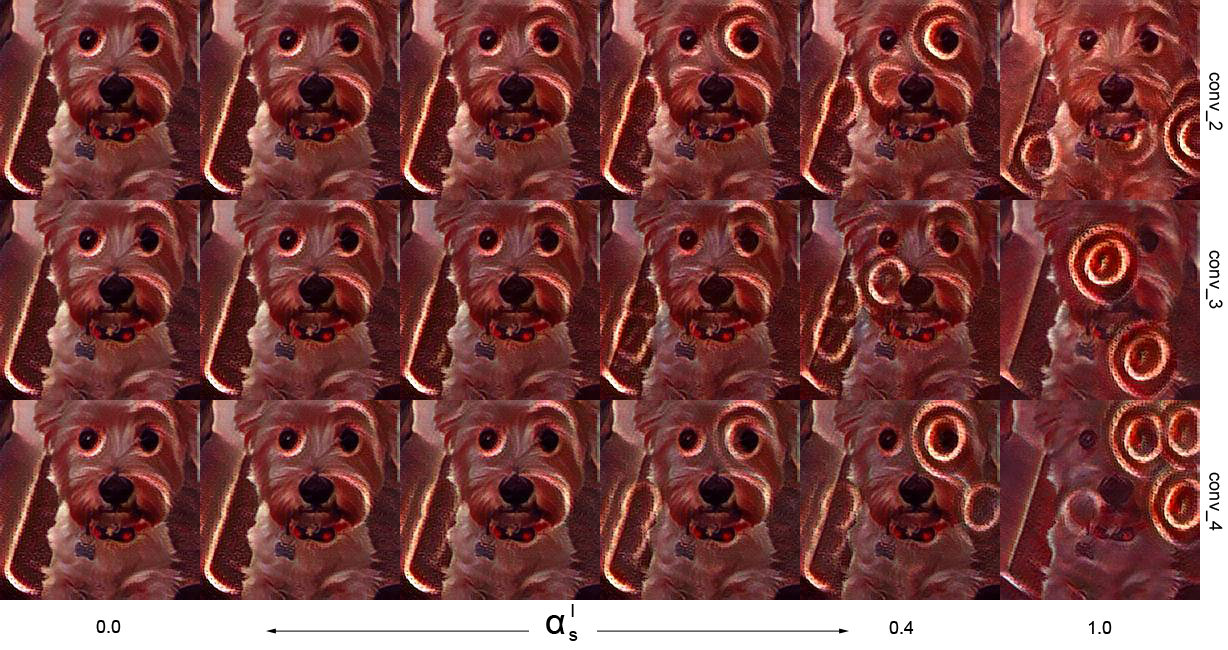
\includegraphics[width=0.49\textwidth, scale=0.1]{fig3_old_small.png}
    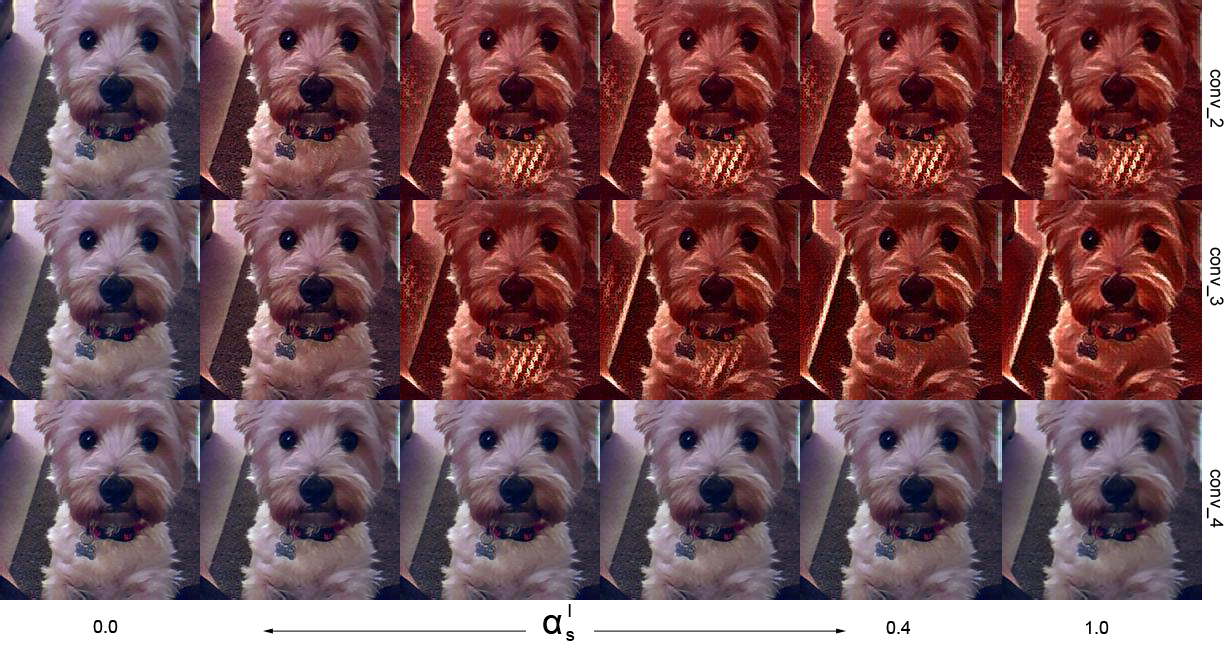
\includegraphics[width=0.49\textwidth, scale=0.1]{fig3_ours_small.png}
    \vspace{-3mm}
    \caption{Truncated reproduction of Figure 3 using NP's (left) and our own implementation (right)}
    \label{fig3}
\end{figure}

The second experiment was to reproduce the effects of combining the styling from several convolution layers (Figure 6). There is no specific result here, however the styling should look different after combining the effects from different layers. Using both Prudnikov's model and the group's model, the input image was stylised based on a combination of layers as shown in Figure \ref{fig6}. Both models did produce distinct stylised images, with Prudnikov's model opting to favour circular style features, whilst the group's model favoured linear features.

\begin{figure}[h!]
    \centering
    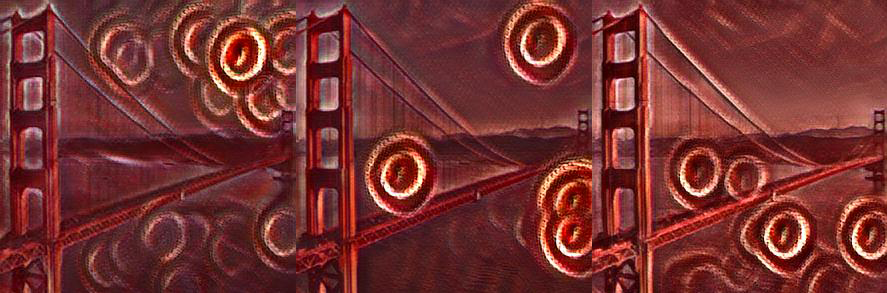
\includegraphics[width=0.49\textwidth, scale=0.1]{fig6_old_small.png}
    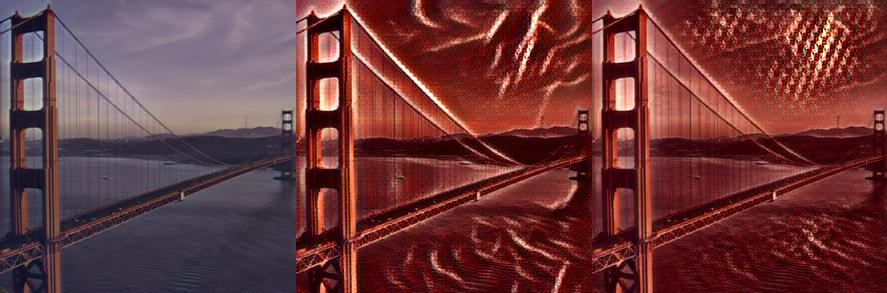
\includegraphics[width=0.49\textwidth, scale=0.1]{fig6_ours_small.png}
    \vspace{-3mm}
    \caption{Truncated reproduction of Figure 6 using NP's (left) and our own implementation (right)}
    \label{fig6}
\end{figure}

\subsection{Effect of noise}\label{ss:noise}
Figure 5 from \cite{babaeizadeh2018adjustable} demonstrates the effect on the images produced by adjusting parameters of the model, adding a few points of Gaussian noise and doing both of these things. The paper specifies that the noise should be produced by multiplying the input image with a white mask, in which fewer than 10 randomly-chosen pixels have been changed to 0 (black). An inverse Gaussian filter is then applied to this mask. Efforts to reproduce the figure using this method using Prudnikov's code were unsuccessful. The tiny amounts of added noise did not affect the final result as much as the paper suggests, and all produced images were identical. The most likely explanation is that the transformations using Prudnikov's code are not sensitive enough for such small changes to make a difference. Experimenting by randomly adding larger noise spots did produce different results, as shown in Figure \ref{gaussnoise}. Reproduction of the figure using this technique demonstrates that the addition of noise to the input image does affect the image produced, though the images produced are not particularly similar to those produced by the original author and the method is different. The same process was carried out using the new model, as shown on the right in Figure \ref{fig5git}. While the inverse Gaussian method of adding noise again didn't make any noticeable difference, there was a substantial difference when adding the black spots as described above. The effect of adding the randomisation is generally less visible using the new model, due to its avoidance of the other model's tendency to obscure details by adding swirls.

\begin{figure}[h!]
    \centering
    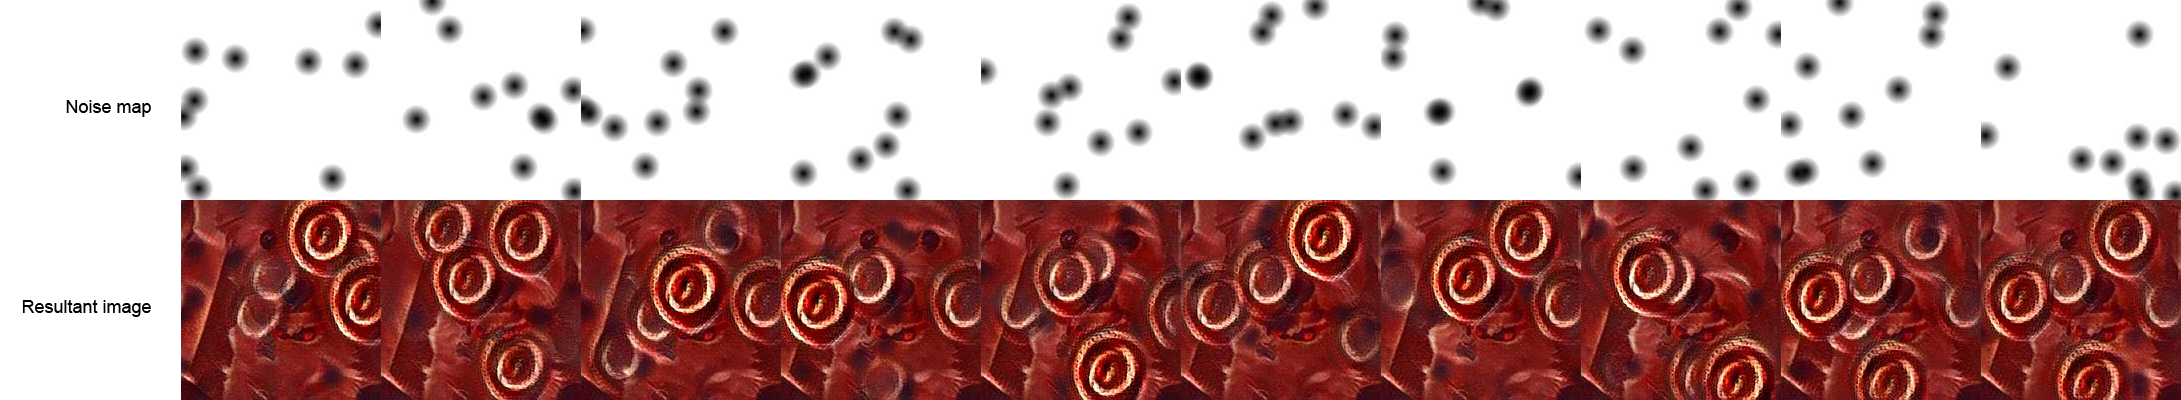
\includegraphics[width=\textwidth, scale=0.1]{non_gauss2.png}
    \vspace{-7mm}
    \caption{Effect of adding noise to the input image}
    \label{gaussnoise}
\end{figure}

\begin{figure}[h!]
    \centering
    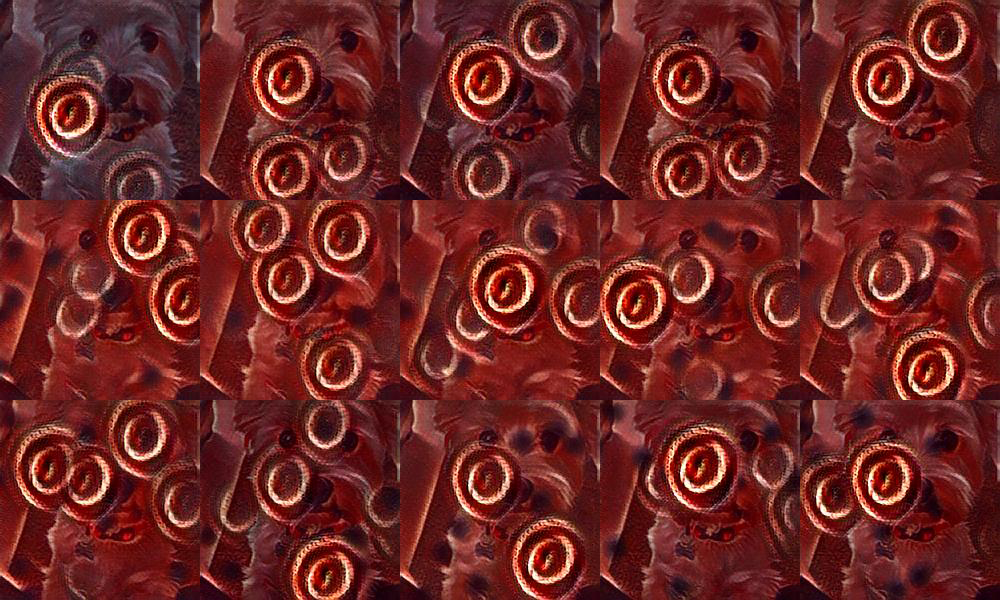
\includegraphics[width=0.49\textwidth, scale=0.1]{fig5git.png}
    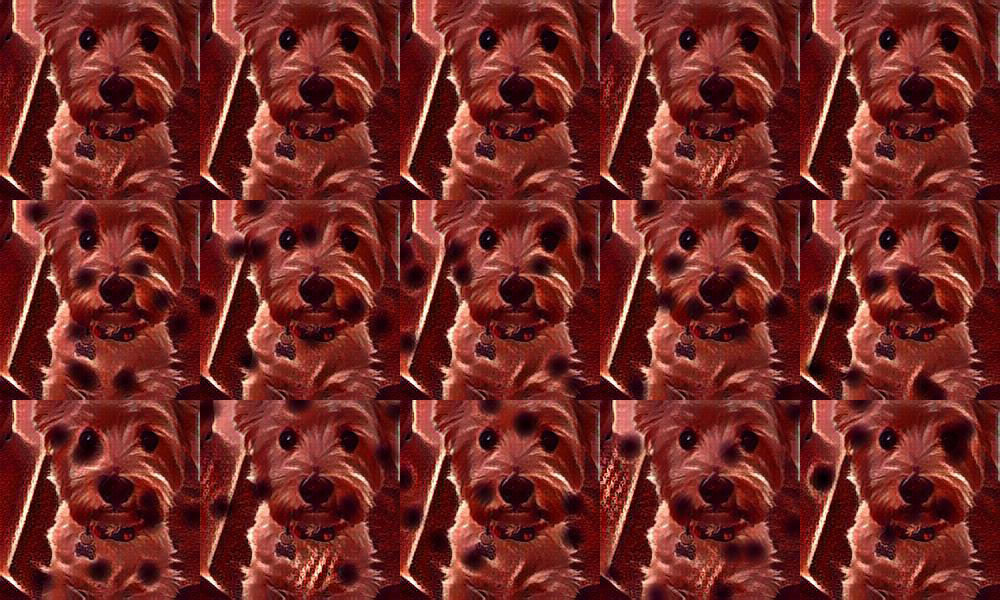
\includegraphics[width=0.49\textwidth, scale=0.1]{fig5own.png}
    \vspace{-3mm}
    \caption{Truncated reproduction of Figure 5 using NP's (left) and our own implementation (right)}
    \label{fig5git}
\end{figure}

\section{Conclusion}
Using the methodology provided by \cite{babaeizadeh2018adjustable}, an Adjustable Real-Time Style Transfer model was implemented, reproducing results to an acceptable level. Likely due to the under-specification in the paper, the reproductions were not completely representative of the original, however they still showed that stylisation of an image can be varied using weights, without retraining the network. Due to computation time to train one style network, testing capabilities were limited when compared to the original paper's.

\bibliography{C:/Users/Carl/Documents/Year4/Semester2/Deep_Learning/Reproducibility_Challenge/Report/DL_report.bib}
\bibliographystyle{iclr2019_conference}
\end{document}